\section{Шардирование}

В данном разделе рассматриваются фундаментальные аспекты шардирования как
ключевого метода горизонтального масштабирования баз данных. Исследуются
базовые принципы распределения данных, проводится сравнительный анализ
вертикального и горизонтального шардирования с практическими примерами их
применения. Особое внимание уделяется системному анализу преимуществ и
ограничений шардированной архитектуры, включая вопросы отказоустойчивости,
производительности и сложности реализации. Завершает раздел обзор основных
методов шардирования с характеристикой их специфических особенностей и областей
эффективного применения.

\subsection{Общая информация}

Шардирование — это подход к организации баз данных, при котором массив данных
делится на части и распределяется по различным узлам (шардам). Шард является
самостоятельным компонентом кластера и для повышения надёжности часто
поддерживает включает не только мастеров, но и реплики — серверы, хранящие
копию данных мастера.

Данная технология становится востребованной, когда система исчерпывает
возможности вертикального масштабирования (усиления мощности одного сервера) и
для дальнейшего роста ей требуется горизонтальное масштабирование (добавление
новых машин).

Популярные онлайн-сервисы со временем неизбежно нуждаются в масштабировании для
увеличения пропускной способности и быстродействия. Когда, например, социальная
сеть разрастается до многомиллионной аудитории, её работа на одном сервере
становится невозможной. Для безопасного и целостного распределения информации
между несколькими серверами применяется шардированная база данных.

\subsection{Виды шардирования}

Выделяют два вида шардирования:

\begin{itemize}
    \item Вертикальное — это вид шардирования, при котором
    данные распределяются по столбцам. Каждый шард в этой схеме хранит
    определенный набор колонок со всеми соответствующими строками. Данный
    подход особенно эффективен в сценариях, когда отдельные столбцы
    запрашиваются значительно чаще остальных.

    В качестве иллюстрации можно рассмотреть базу данных интернет-магазина,
    содержащую обширную информацию о товарах и клиентах. Для повышения
    производительности её можно разделить на два шарда: первый будет
    специализироваться на данных о покупателях, а второй — на информации о
    продуктах. Это позволит системе загружать только те столбцы, которые
    необходимы для выполнения конкретного запроса, оптимизируя таким образом
    использование ресурсов. Пример архитектуры вертикального шардирования
    представлен на рисунке~\ref{fig:fig01}.

\begin{figure}
  \centering
  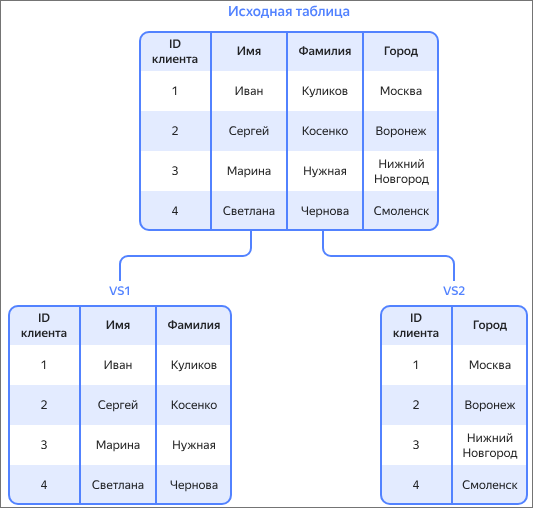
\includegraphics[scale=0.35]{inc/vertical-sharding.png}
  \caption{Вертикальное шардирование}
  \label{fig:fig01}
\end{figure}
    \item Горизонтальное — это вид шардирования, основанный на разделении строк
    таблицы в соответствии с определёнными правилами или ключами. При таком
    подходе каждый шард обладает идентичной схемой столбцов, но содержит
    уникальные наборы записей. Данная технология обеспечивает эффективное
    распределение операций чтения и записи между несколькими независимыми
    серверами, повышая общую производительность и отказоустойчивость системы.

    В качестве практического примера можно рассмотреть базу пользователей
    социальной сети. Для снижения нагрузки на инфраструктуру разработчики
    применяют горизонтальное партиционирование, используя хеш-функцию от
    первичного ключа (например, ID пользователя) для определения целевого шарда
    для каждой новой записи. Этот подход гарантирует равномерное распределение
    данных и запросов по всем узлам кластера. Пример реализации горизонтального
    шардирования демонстрируется на рисунке~\ref{fig:fig02}.

\begin{figure}
  \centering
  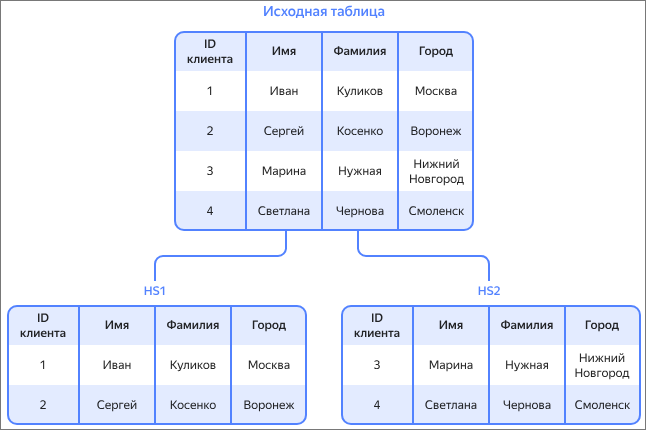
\includegraphics[scale=0.35]{inc/horizontal-sharding.png}
  \caption{Горизонтальное шардирование}
  \label{fig:fig02}
\end{figure}
\end{itemize}

\subsection{Преимущества и недостатки шардирования}

Когда монолитная база данных достигает пределов вертикального масштабирования,
шардирование становится эффективным решением для дальнейшего роста. Данная
архитектура предоставляет следующие преимущества:

\begin{itemize}
    \item \textbf{Преодоление аппаратных ограничений}. Популярные сервисы часто
    упираются в физические лимиты оборудования. Шардирование позволяет
    распределить информацию среди нескольких серверов, обеспечивая тем самым
    горизонтальное масштабирование и возможность практически неограниченного
    расширения.

    \item \textbf{Повышение отказоустойчивости}. Поскольку шарды физически
    размещаются на разных серверах, выход из строя одного из них не приводит к
    полному отказу системы. Это означает, что вместо полной недоступности
    сервиса может перестать функционировать лишь его некоторая часть, что
    значительно повышает надежность.

    \item \textbf{Увеличение производительности}. Монолитные базы данных часто
    страдают от конкуренции запросов, что снижает общую скорость работы.
    Шардирование распределяет нагрузку между узлами, что позволяет увеличить
    пропускную способность системы и ускорить обработку данных.
\end{itemize}

Несмотря на свою мощь, шардированная архитектура имеет ряд существенных
недостатков, которые делают её применение целесообразным не во всех ситуациях.

\begin{itemize}
    \item \textbf{Высокая сложность внедрения и сопровождения}. Процесс
    шардирования критически важен, и ошибки на этапе проектирования могут
    привести к потере или повреждению данных. Кроме того, разработка
    усложняется, так как исчезает единая точка входа для работы с данными, и
    команде приходится оперировать множеством изолированных сегментов.

    \item \textbf{Риск несбалансированной нагрузки}. Распределение данных может
    оказаться неравномерным, если критерии шардирования выбраны неудачно.
    Это приводит к ситуации, когда один шард (например, с данными популярных
    пользователей) обрабатывает большую часть запросов, создавая «горячую
    точку». Для устранения такой несбалансированности часто требуется
    трудоемкая процедура решардинга, часто сопровождающаяся простоем.

    \item \textbf{Снижение эффективности сложных запросов}. Операции, которые
    требуют агрегации данных из нескольких шардов (например, JOIN'ы),
    выполняются значительно медленнее из-за необходимости сетевого
    взаимодействия с разными серверами и последующего объединения результатов.
    Это делает такие запросы более ресурсоемкими по сравнению с выполнением в
    рамках единой базы данных.
\end{itemize}

\subsection{Методы шардирования данных}

В практике распределённых баз данных применяются различные подходы к
шардированию, каждый из которых обладает специфическими характеристиками. Выбор
оптимальной стратегии зависит от конкретных требований и архитектурных
особенностей системы. Наиболее распространённые методы включают:

\begin{itemize}
    \item \textbf{Хеш-шардирование} — распределение данных между шардами
    осуществляется на основе вычисленного хеш-значения от ключа записи. Данный
    метод обеспечивает равномерное распределение нагрузки и высокую доступность
    системы, но осложняет выполнение запросов по диапазонам значений.

    \item \textbf{Диапазонное шардирование} — разделение данных производится
    согласно заданным интервалам значений ключевых атрибутов. Подход отличается
    простотой реализации и эффективностью при выполнении запросов в пределах
    определённого диапазона, однако может приводить к неравномерному
    распределению нагрузки между шардами.

    \item \textbf{Круговое шардирование} — шарды организуются в логическое
    кольцо, где каждый узел отвечает за определенный сегмент данных. Запросы
    маршрутизируются в соответствии с позицией шарда в кольцевой структуре.
    Метод обеспечивает равномерное распределение запросов, но требует сложной
    процедуры перераспределения данных при изменении количества шардов.

    \item \textbf{Динамическое шардирование} — система автоматически адаптирует
    структуру хранения в зависимости от текущей нагрузки и объема данных.
    Несмотря на высокую гибкость и масштабируемость, данный подход требует
    сложной системы мониторинга, балансировки нагрузки и тщательно продуманной
    архитектуры.
\end{itemize}

